\documentclass[11pt, a4paper]{article}
\input{preamble.tex}
\switchlang{en}
\begin{document}

\title{1994 -- Trinity Mariqua Mouse}
\date{}
\maketitle
\selectlanguage{english}

The Trinity Mariqua Mouse was released in 1994 for the Japanese market by the Miyuki Electronic Design company. Following in the footsteps of the Prohance family of mice and trackballs from 1989, the Mariqua Mouse embodies the idea of placing additional buttons on the mouse body, which, according to the developers, eliminates the need for the user to frequently move hand from the mouse to the keyboard and back.

The Trinity Mariqua was released in two color variants (fig. \ref{fig:TrinityPic}): a metallic-red body with black accents, and a white body with gray accents.

\begin{figure}[h]
    \centering
    
\includegraphics[scale=0.55]{1994_mariqua_mouse/pic_30.jpg}
    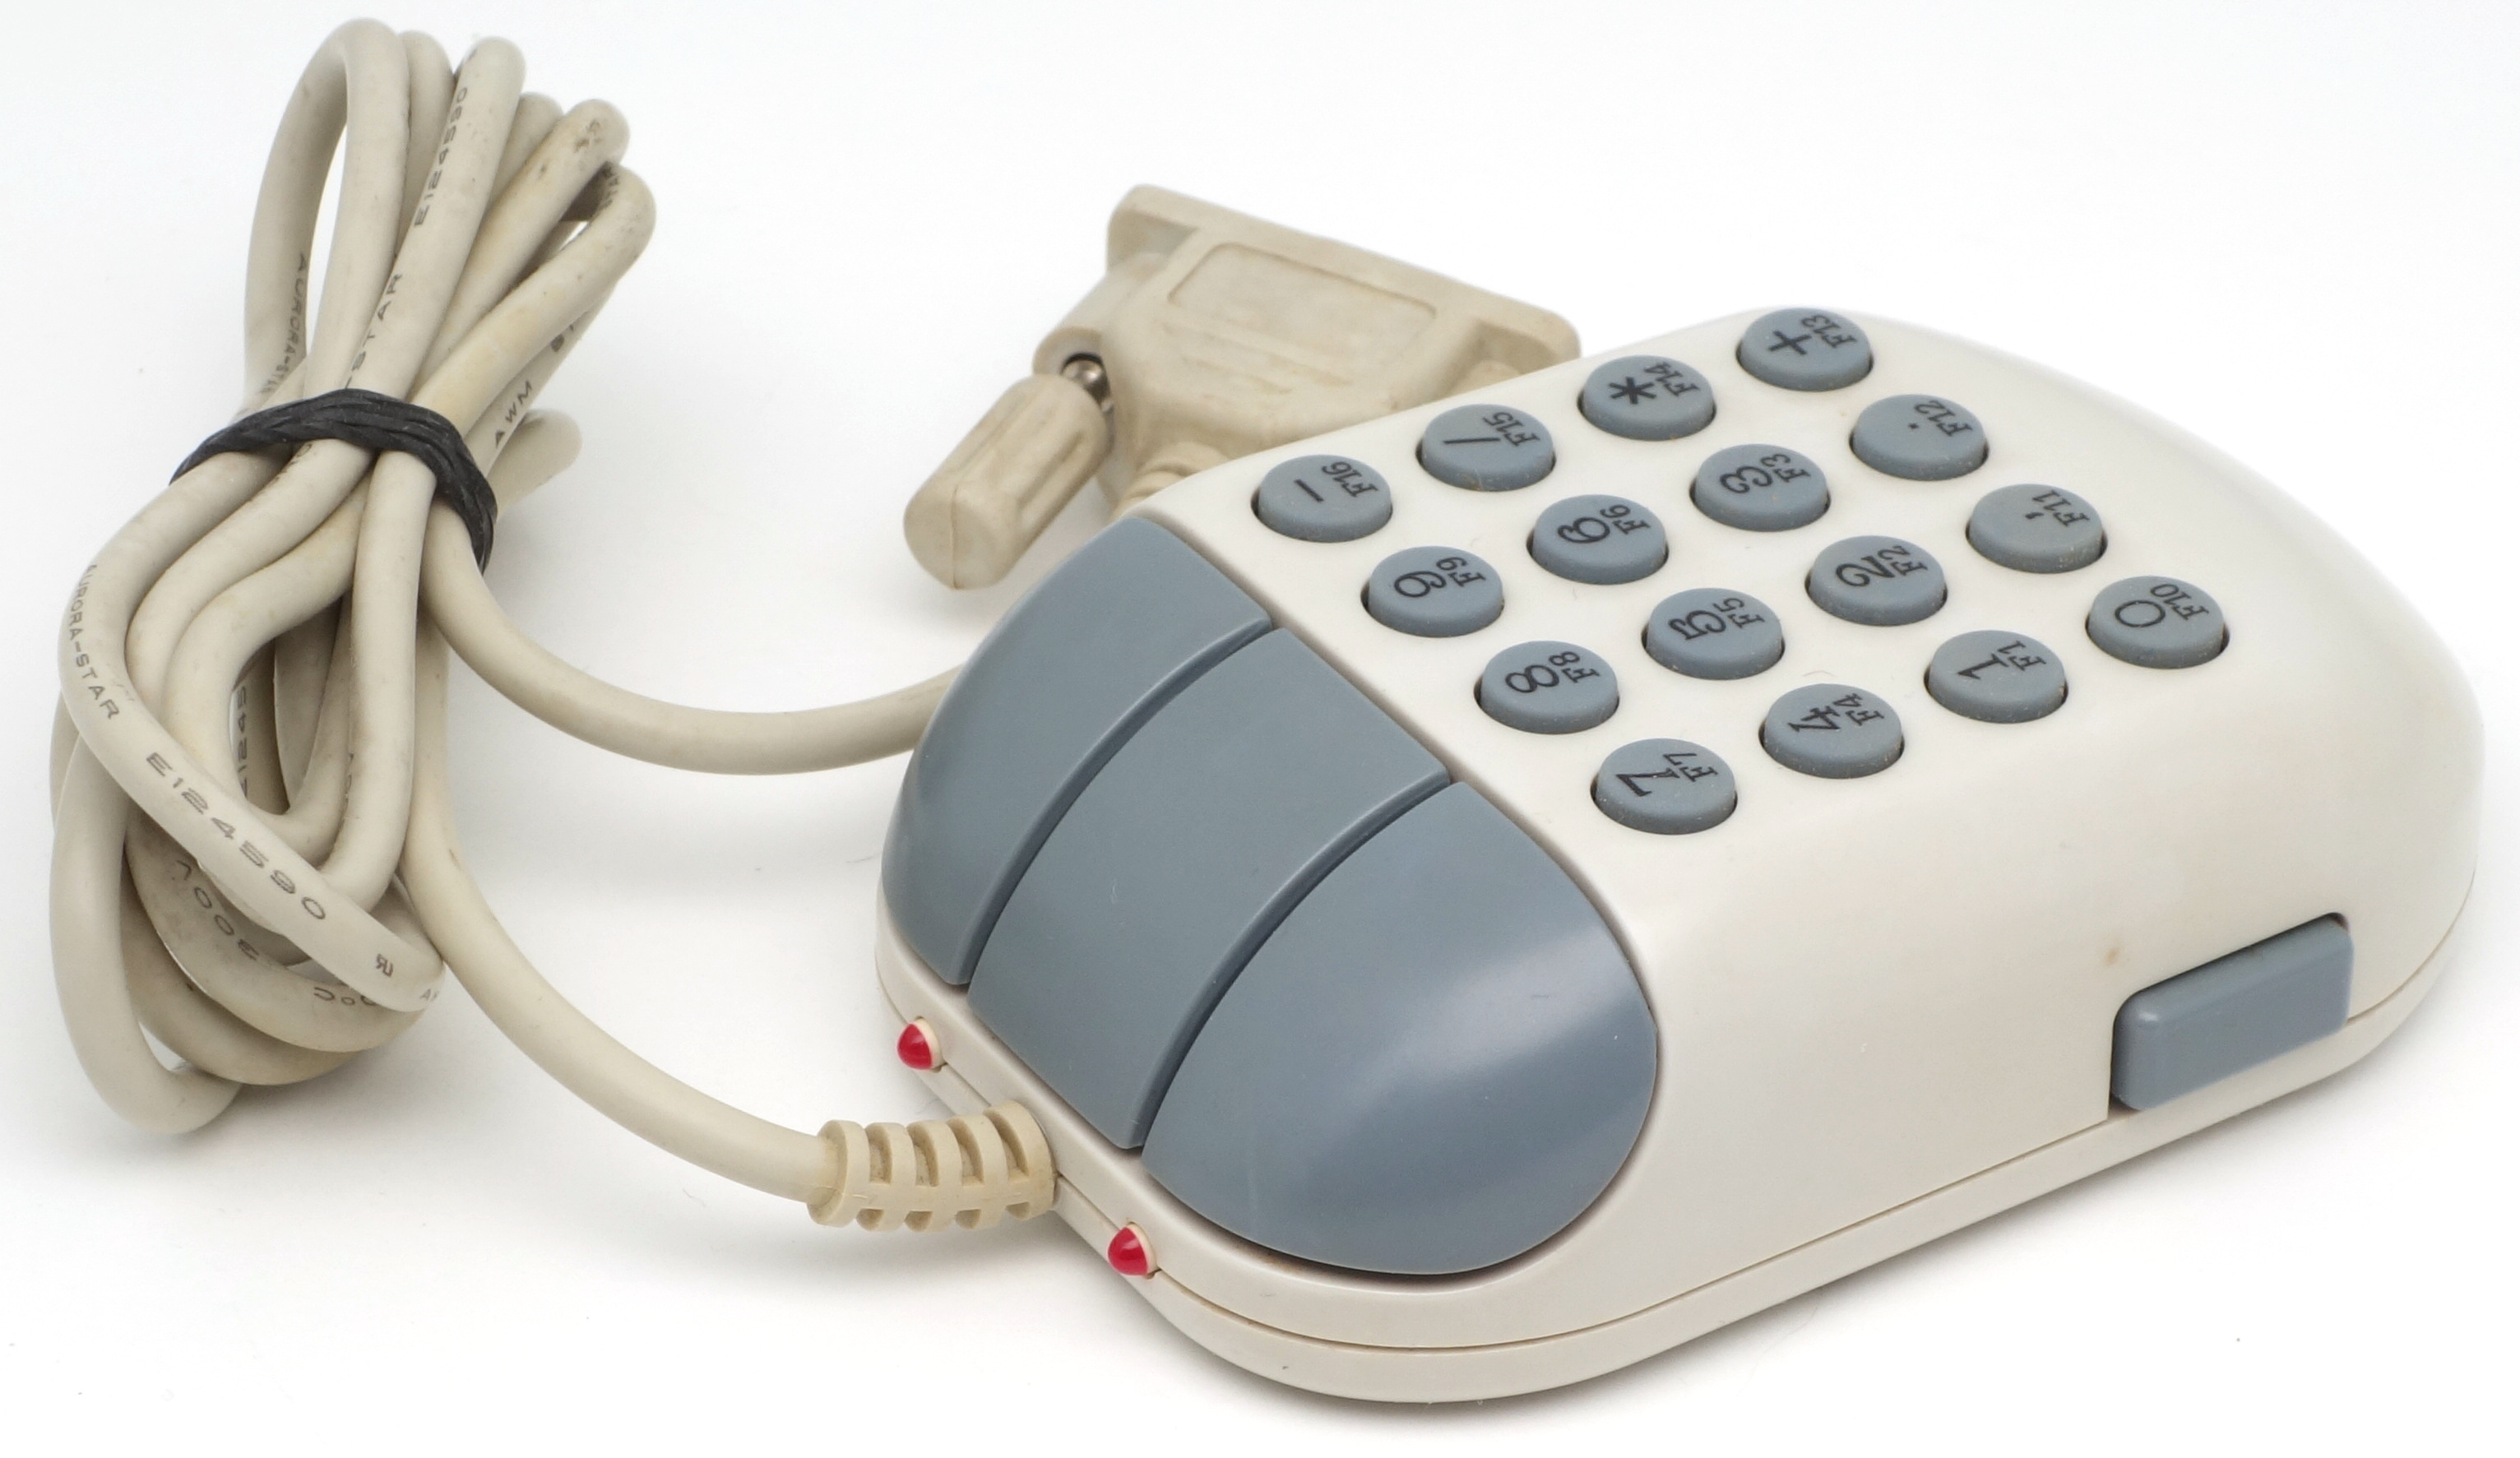
\includegraphics[scale=0.5]{1994_mariqua_mouse/pic_white_30.jpg}
    \caption{Trinity Mariqua Mouse}
    \label{fig:TrinityPic}
\end{figure}

On the underside of the case (fig. \ref{fig:TrinityTopBottom}) are a rotating ring for removing the ball and cleaning the mouse, a label with technical data, and four low-friction pads. On the top side are three fairly large buttons extending onto the front of the mouse case, as well as 16 miniature round buttons that serve as a numeric keypad and function keys. On the sides of the case are two more rectangular buttons. Additionally, on the front of the case is a ribbed sleeve that protects the cable from mechanical damage where it exits the case, as well as two LEDs surrounding it.

\begin{figure}[h]
    \centering
    
\includegraphics[scale=0.7]{1994_mariqua_mouse/top_15.jpg}
    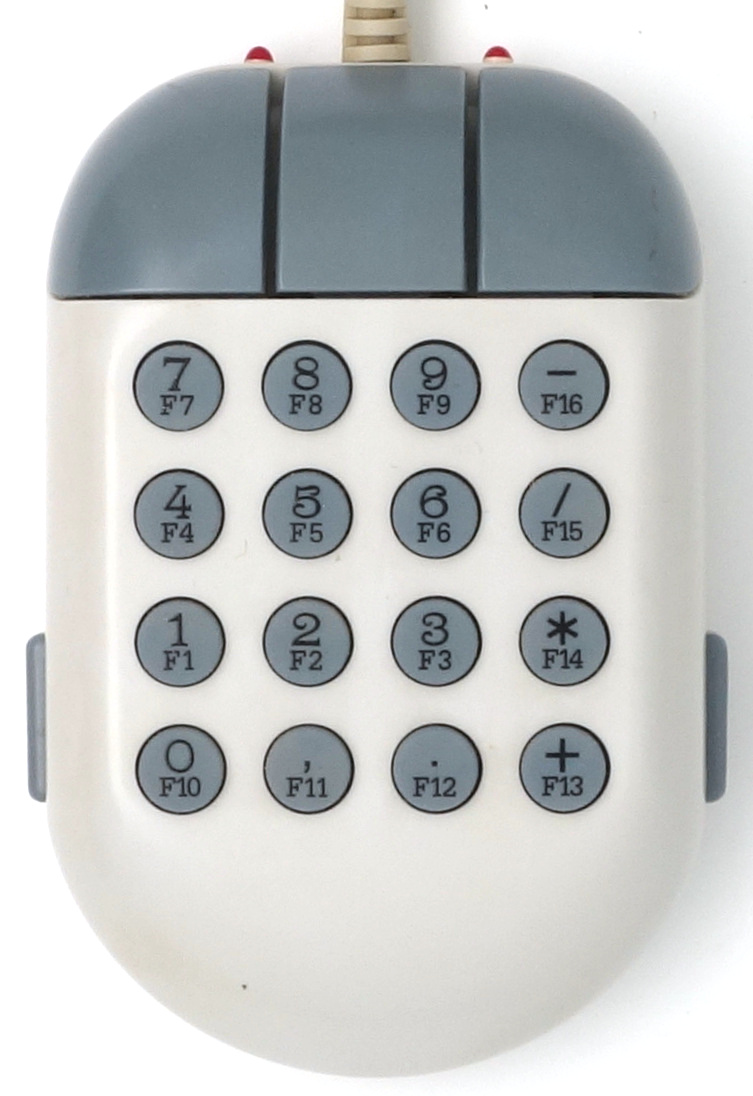
\includegraphics[scale=0.7]{1994_mariqua_mouse/top_white_30.jpg}
    
\includegraphics[scale=0.68]{1994_mariqua_mouse/bottom_15.jpg}
    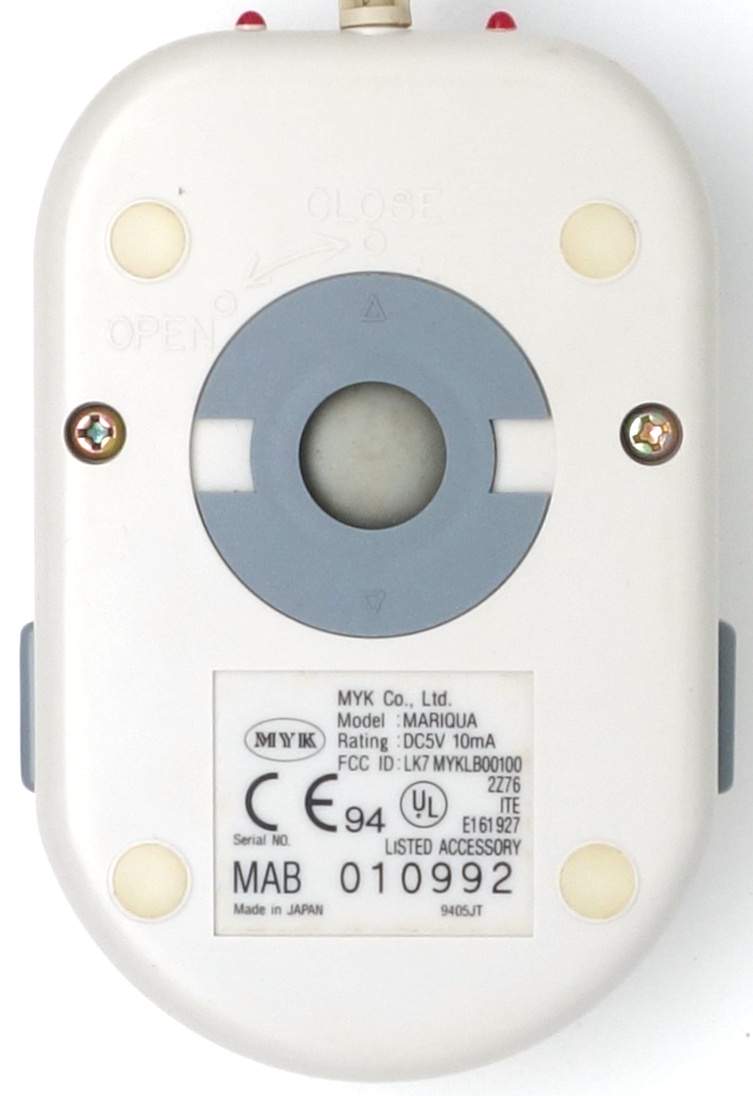
\includegraphics[scale=0.69]{1994_mariqua_mouse/bottom_white_30.jpg}
    \caption{Mariqua Mouse, top and bottom views}
    \label{fig:TrinityTopBottom}
\end{figure}

This particular Trinity Mariqua Mouse sample connects to the computer via a serial interface, and its three big buttons perform the standard function of the left, middle, and right mouse buttons.

However, there were also mouse variants with an ADB interface designed for use with Apple computers.
In these, the left button acted as the primary (or, in the case of Apple, only) mouse button, the right button acted as a click trigger to facilitate dragging (one click generated a primary button press event, the second a release event), and the middle button triggered a double-click of the primary mouse button \cite{info_1}.

\begin{figure}[h!]
    \centering
    
\includegraphics[scale=0.34]{1994_mariqua_mouse/size_30.jpg}
    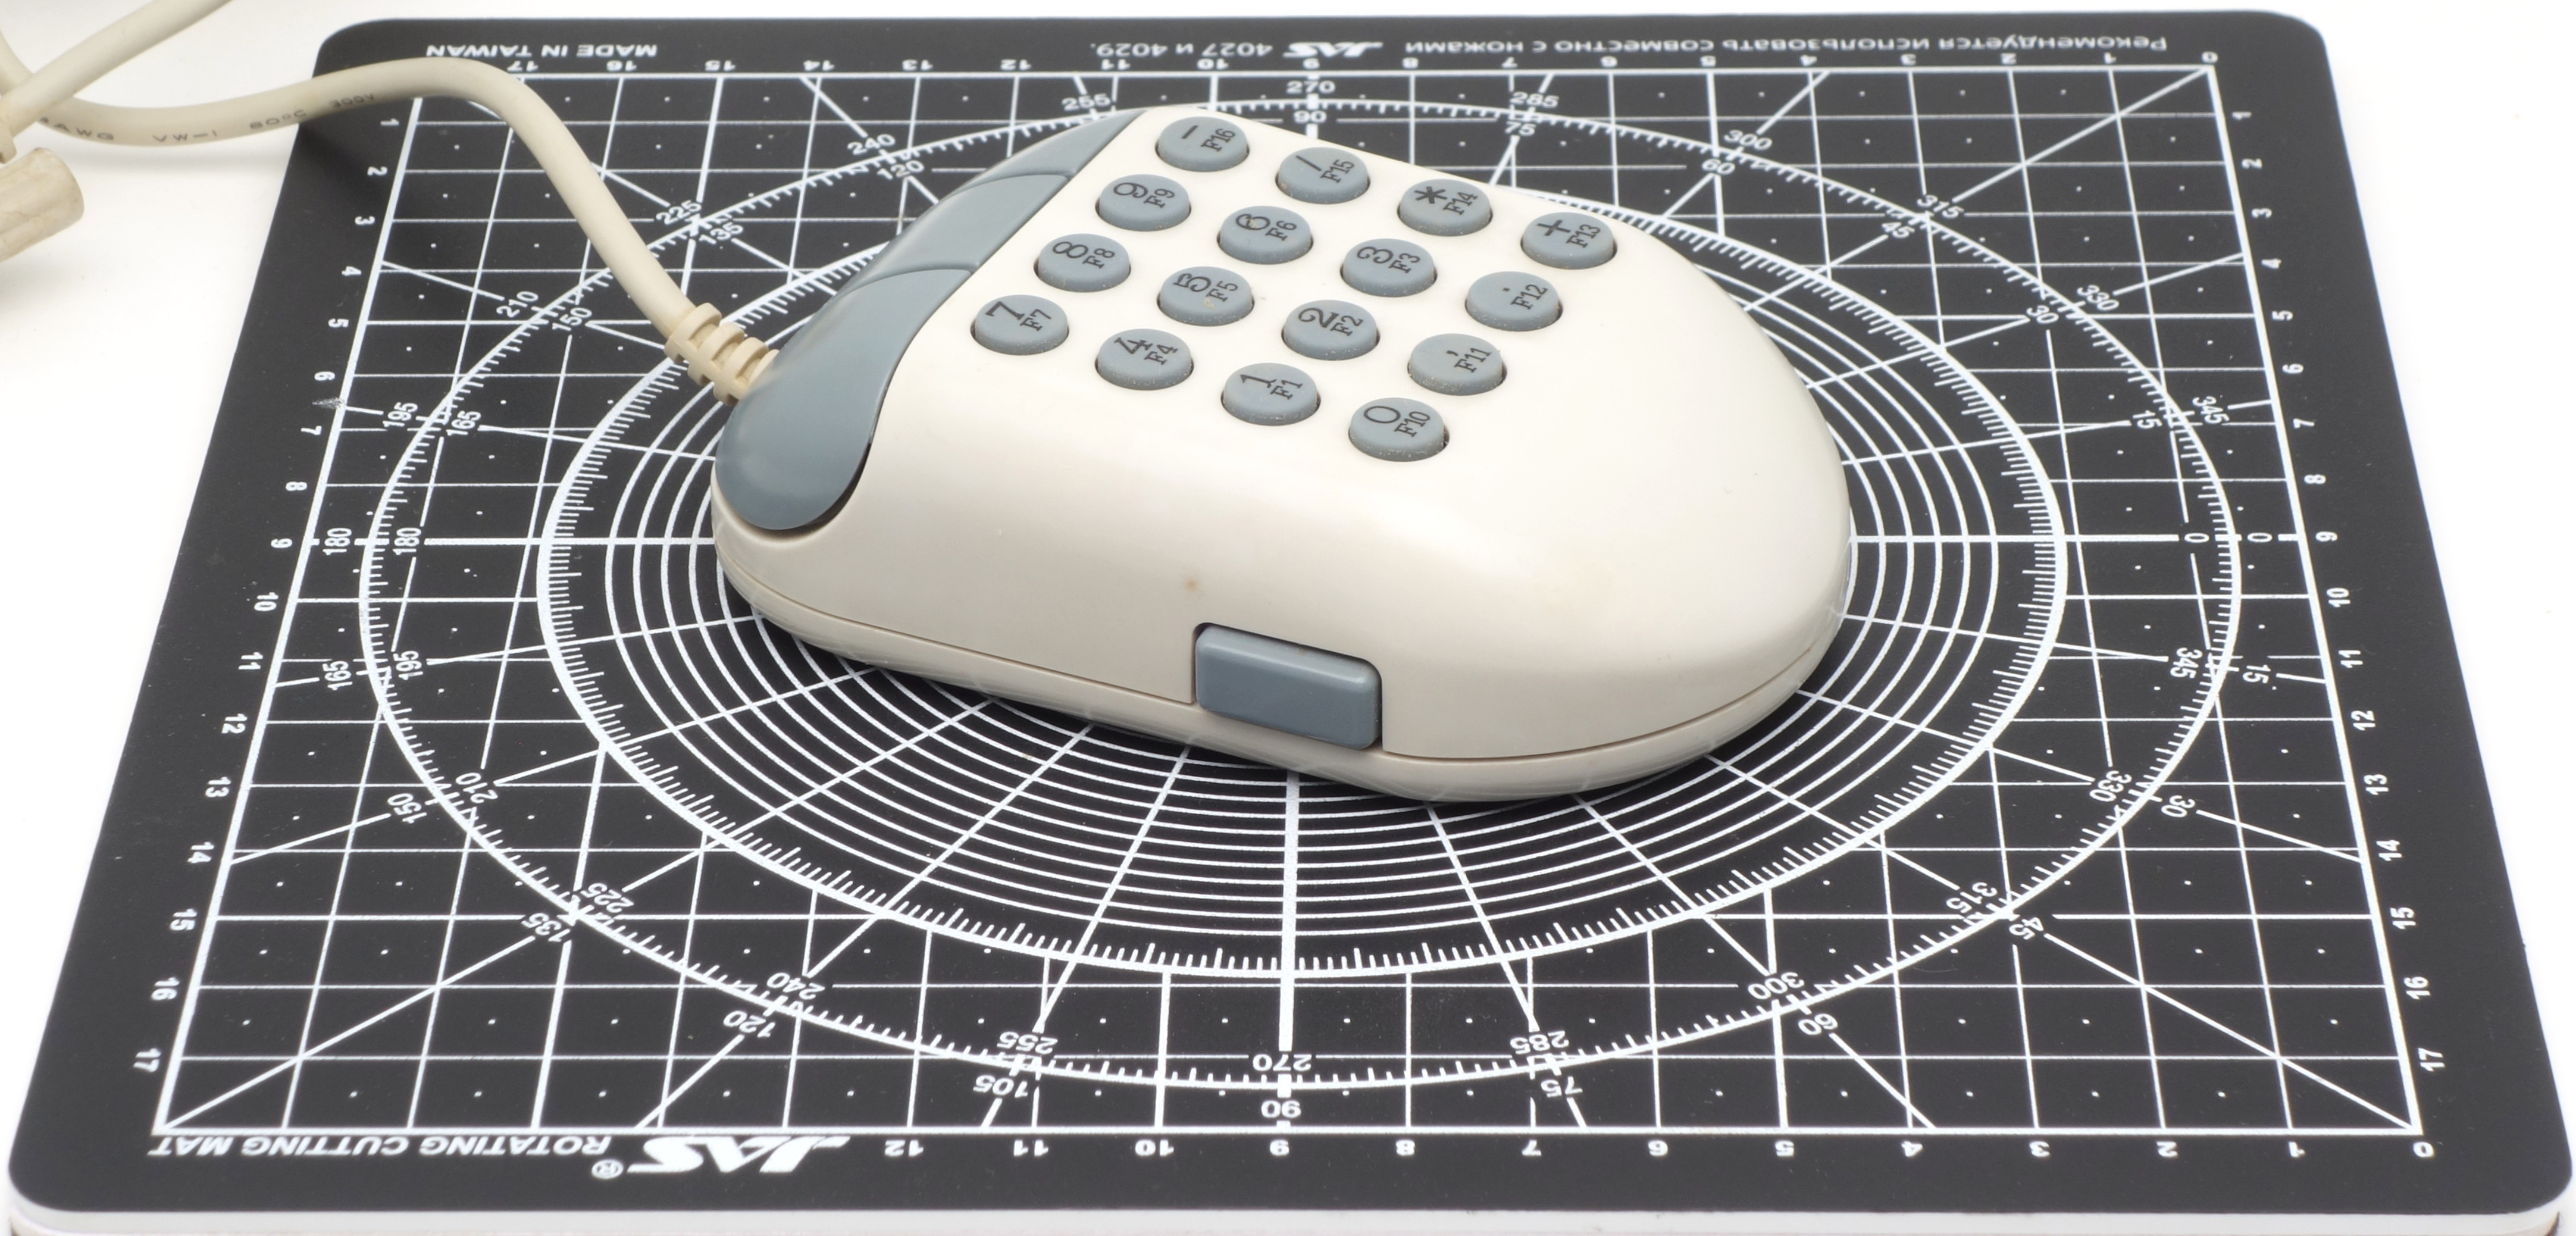
\includegraphics[scale=0.5]{1994_mariqua_mouse/size_white_15.jpg}
    \caption{Mariqua Mouse on a graduated pad with a grid step of 1~cm}
    \label{fig:TrinitySize}
\end{figure}

The mouse's keyboard is disabled by default to prevent accidental keystrokes. To activate the numeric keypad, the user must press the left side button, which also turns on the LED on the front of the device (the convenience of this indicator method is questionable, as the LEDs are invisible when the mouse is in its normal position).

The numeric keypad includes 10 keys, represented by numbers from 0 to 9, mathematical operation keys “+”, “-”, “*”, “/”, and a decimal sign “,”. Each press of these keys produces a beep, which can also cause discomfort with frequent use.

To exit the numeric keypad mode, the user must press the left side button again.

The right side button activates the keys' secondary function (in this mode, they function as keyboard function keys) and also allows the user to switch between modes. It's important to note that pressing the right side button activates this mode, while pressing any of the round buttons on the top of the case deactivates it, returning the device to mouse mode. This is because function keys typically don't require repeated use \cite{info_1}.

\begin{figure}[h]
    \centering
     
\includegraphics[width=\textwidth]{1994_mariqua_mouse/hand_30.jpg}
    \caption{Mariqua Mouse with a human hand model}
    \label{fig:TrinityiHand}
\end{figure}

The figure \ref{fig:TrinityiHand} shows a typical palm position on the mouse body. It should be acknowledged that, with the exception of the tiny round buttons, the device is a fairly comfortable compact mouse with a moderately streamlined body shape, typical of the mid-90s trend. Thanks to the symmetrical design of its body, the device is equally suitable as a mouse for left-handed and right-handed users. Pressing the left side and right side buttons is less comfortable when the mouse is covered with a palm, probably to avoid accidental presses, but in any case that is not a big problem taking into account the fact that they are related to the ``keyboard'' part, which is far from being very convenient.

The mouse's internal structure is shown in the figure \ref{fig:TrinityInside}. Besides the additional numeric keypad, this mouse features a standard optomechanical cursor control unit with a normal motion detection unit from the mid-1990s. The bras rollers allow to add this device to the class of mice with good durability of the mechanical unit. The numeric keypad is located on a separate board, which is connected to the main board via a flexible ribbon cable.

\begin{figure}[h]
    \centering
    
\includegraphics[scale=0.8]{1994_mariqua_mouse/inside_30.jpg}
    \caption{Mariqua Mouse disassembled}
    \label{fig:TrinityInside}
\end{figure}

\begin{thebibliography}{9}
\bibitem {info_1} Dandumont P. La souris ADB qui fait clavier avec bips et feux de position - Le journal du lapin \url{https://www.journaldulapin.com/2022/06/06/souris-clavier-adb/}
\end{thebibliography}

\end{document}
